\section{系统架构}
\label{sec:architecture}

\begin{figure}
\centering
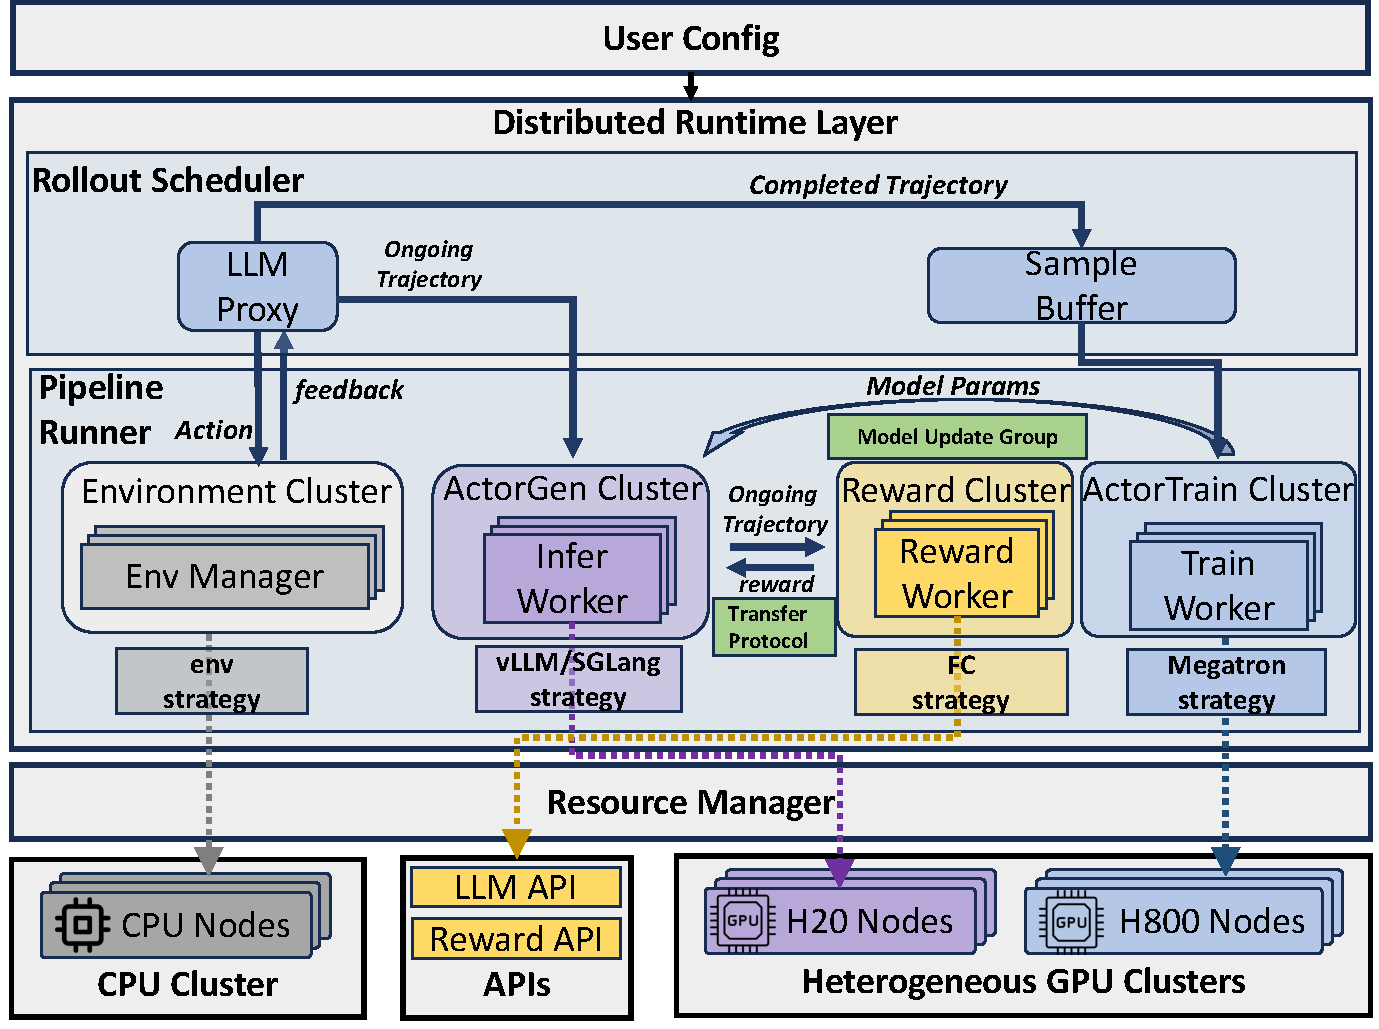
\includegraphics[width=0.9\linewidth]{figs/overview/sys_arch_osdi_updated.pdf}
\caption{\SystemName{} 的系统架构。}
\label{fig:sys_arch}
\end{figure}

我们用约 6 万行 Python 从零实现了 \SystemName{}。\autoref{fig:sys_arch} 展示了它的两层结构：分布式运行时层和资源管理器。\SystemName{}首先解析用户配置，并在分布式运行时之上构造训练流水线。运行时包含 rollout 调度器，用于管理 rollout 执行流程；还包含负责分布式计算与通信的 \texttt{Cluster} 运行时。资源管理器则从共享资源池中为各类 worker 分配异构资源。

\noindent\textbf{Rollout Scheduler。}
调度器通过管理每条轨迹的生命周期来控制 rollout 阶段。\texttt{LLMProxy} 与多个环境管理器交互，并把进行中的轨迹路由到合适的推理 worker。完成的轨迹被加入 \texttt{SampleBuffer}，供后续训练使用。

\noindent\textbf{Pipeline Runner。}
Pipeline runner 由多个 \texttt{Cluster} 组成，每个 \texttt{Cluster} 在 agentic RL 中承担不同角色，如 reward、environment 或 training。每个集群使用选定执行策略（例如 vLLM~\cite{vllm}、Megatron~\cite{shoeybi2019megatron}、Function Compute~\cite{alibaba_function_compute}）组织一组 worker 执行特定类型的分布式计算。\texttt{Cluster} 之间通过 Ray 的 \texttt{ObjRef}~\cite{ray} 交换轨迹，从而避免频繁复制数据，并以延迟物化方式隐藏传输开销。对于模型权重同步，每个 \texttt{Cluster} 暴露 \texttt{model\_update\_group} 接口，并结合 NCCL~\cite{nccl} 与 Mooncake~\cite{qin2024mooncake} 等高吞吐传输引擎，利用 NVLink、InfiniBand 与以太网高效完成同步。

\noindent\textbf{Resource Manager。}
资源管理器通过持久化元数据存储维护系统关键状态，包括运行时状态、集群资源可用性以及服务 API 的可用性。当收到 worker 部署请求时，它首先查询元数据验证请求，再把所需资源或外部服务绑定到相应 worker 上。
